%
% This work may be distributed and/or modified under the
% conditions of the LaTeX Project Public License, either version 1.3
% of this license or (at your option) any later version.
% 
% The Current Maintainer of this work is P. S. Eduardo.
%
% This work consists of the file poli.cls.
%% -----------------------------------------------------------------
% Escola Politécnica UFRJ ECI LaTeX Template
% Version: 1
% Author: Filipe Santos Pacheco Prates
% email: filipespprates@gmail.com
% Base: P. S. Eduardo's
%%------------------------------------------------------------------
\documentclass[grad,pdftex]{poli}
\usepackage[utf8]{inputenc}
\usepackage{amsmath,amssymb}
\usepackage{float}
\usepackage{multirow}
\usepackage{longtable}
\usepackage{tikz}
\usepackage{listings}
\lstdefinelanguage{JavaScript}{
  keywords={typeof, new, true, false, catch, function, return, null, catch, switch, var, if, in, while, do, else, case, break},
  keywordstyle=\color{blue}\bfseries,
  ndkeywords={class, export, boolean, throw, implements, import, this},
  ndkeywordstyle=\color{darkgray}\bfseries,
  identifierstyle=\color{black},
  sensitive=false,
  comment=[l]{//},
  morecomment=[s]{/*}{*/},
  commentstyle=\color{purple}\ttfamily,
  stringstyle=\color{red}\ttfamily,
  morestring=[b]',
  morestring=[b]"
}

\lstset{
   language=JavaScript,
   backgroundcolor=\color{lightgray},
   extendedchars=true,
   basicstyle=\footnotesize\ttfamily,
   showstringspaces=false,
   showspaces=false,
   numbers=left,
   numberstyle=\footnotesize,
   numbersep=9pt,
   tabsize=2,
   breaklines=true,
   showtabs=false,
   captionpos=b
}


\usetikzlibrary{shapes,arrows,chains,positioning}
\usepackage{enumitem}
\usepackage{indentfirst}
\usepackage{array}
\usepackage{diagbox}
\usepackage{natbib}
%\usepackage[alf, bibjustif]{abntex2cite}

\makelosymbols
\makeloabbreviations

\begin{document}
  \title{Interface de 'Perfis e Listas' para Sistema Gerenciador de Banco de Dados em Grafo}
  \foreigntitle{}
  \author{Filipe}{S. P. Prates}
  \advisor{Prof.}{Daniel}{R. Figueiredo}{Ph.D.}
  %\coadvisor{Prof.}{Nome}{Sobrenome}{D.Sc.}
  \examiner{Prof.}{Nome Completo}{Ph.D.}
  \examiner{Prof.}{Nome Completo}{D.Sc.}
  %\examiner{Prof.}{Nome Completo}{D.Sc.}
  \department{ECI} %UTTILIZE A SIGLA DO SEU DEPARTAMENTO MODIFICAR OS NOMES DE CURSO, DEPARTAMENTO E OBTENÇÃO DE GRAU (Obs: caso tenha algum equívoco nesses argumentos, necessário modificar o arquivo poli.cls no local que faz a leitura deste argumento)
  \date{2}{2023}
  \keyword{keyword1}
  \keyword{keyword2}
  \keyword{keyword3}
  \keyword{keyword4}
  \maketitle

  \frontmatter
  \include{Pre-textual/dedic}
  \chapter*{Agradecimentos}

Agradeço as minhas conexões.

Obrigado em especial ao meu irmão Bruno, meu pai Antonio João, minha mãe Jacqueline, minha vó Dorita, meus Professores, em especial ao Daniel, ao Fernando e o Bernard (e o Luis) por terem disponibilizado um ambiente de criação, a Rô e a Erica (e o Andy e outros tantos) que tankaram o suporte, ao Cadu pelas conversas de Design, e os meus amigos Pedro, Bernardo, Nas, Ian, Josue, da escalada, e todos os muitos outros que me influenciaram.
  \begin{abstract}

Descrição de uma aplicação intuitiva para gerenciamento de dados em um banco de dados em grafo.  \textit{highlights} 

\end{abstract}


  \begin{foreignabstract}

@placeholder english abstract

\end{foreignabstract}


  \tableofcontents
  \listoffigures
  \printlosymbols
  \printloabbreviations

  \mainmatter
    \chapter{Introdução}

\section{Motivação}

Gerenciar adequadamente os dados armazenados em um banco de dados é fundamental para qualquer sistema de informação. Tal gerenciamento precisa eficiente e intuitivo, de maneira a evitar alterações equivocadas e garantir que os usuários do sistema interajam com dados atualizados e corretos.

Com esse objetivo foram desenvolvidos diferentes interfaces para sistemas de gerenciamento de bancos de dados, com formulários relacionados {a} estrutura de tabelas definidos no schema do banco, e possibilidade de interagir com os dados através de uma linguagem de DCL (Data Control Language / Linguagem de Controle de Dados). Soluções como phpMyAdmin, SQL Server Management Studio, ou o Oracle RDBMS trazem essas funcionalidades, porém exclusivamente para bancos de dados SQL.

Para bancos de dados em grafo, no entanto, em especial o Neo4j Database, as ferramentas de gerenciamento de dados disponíveis se limitam à interações diretas por DCL (Neo4j Browser). Sendo assim, geram abertura para alterações equivocadas nos dados e não permitem uma fácil visualização e gerenciamento intuitivo dos dados, especialmente quando utilizados por usuários ingênuos ao schema.

\section{Contribuição}

O presente TCC apresenta uma interface de gerenciamento de dados para bancos de dados Neo4j, através de uma API em Graphql, com foco na visualização, navegação e gerenciamento intuitivo dos dados do grafo armazenado. A interface recebe o schema do banco de dados e gera um ambiente de "Perfis e Listas", que permite a criação e edição de nós, seus relacionamentos, e os dados de cada um destes. Hoje o sistema é usado amplamente por mais de 30 colaboradores principalmente dos times de Qualidade, Desenvolvimento, Suporte e Educacional da empresa para qual foi desenvolvido.

O trabalho documenta o funcionamento e a arquitetura do sistema, tanto a interface do usuário, que é gerada através de componentes reutilizáveis e as ferramentas Nuxt.js, Vue.js e Apollo Client, como a camada intermediária que conecta a interface ao banco de dados. Para tal, utiliza-se o o Node.js, Express.js, e a biblioteca oficial do Neo4j que conecta o banco de dados à uma API em GraphQL, @neo4j/graphql.

A interface do usuário segue uma dinâmica de navegação diferente, onde é mapeado o isomorfismo de um nó e seus vizinhos com uma página de perfil, suas abas e seus elementos, de maneira que conseguimos gerar uma página de perfil para cada um dos nós no banco e assim navegar facilmente através de suas relações para os perfis de outros nós - alterando ou acrescentando dados arbitrariamente no processo.

\section{Organização}

Este TCC está estruturado da seguinte forma:
\begin{itemize}
  \item Soluções existentes de gerenciamento de dados para bancos de dados Neo4j, explicitando a falta de uma solução como a proposta no trabalho.
  \item Um resumo das principais ferramentas e tecnologias utilizadas no desenvolvimento do sistema proposto.
  \item Uma descrição do funcionamento das partes do sistema.
  \item Como o sistema é utilizado na empresa Jovens Gênios
\end{itemize}

OBS: O domínio dos dados da Jovens Gênios consiste principalmente das estruturas escolares (Redes, Escolas, Turmas), as pessoas envolvidas no processo de ensino-aprendizagem (Professores, Gestores, Alunos), além de conteúdos didáticos, organizados numa hierarquia em árvore, uma para cada disciplina definida na BNCC (Base Nacional Comum Curricular).

    \chapter{Trabalhos Relacionados}
\label{chap2}

\section{Soluções existentes de interação com o banco de dados}

\subsection{Neo4j Browser}
A principal ferramenta utilizada para interagir com os dados no banco de dados Neo4j é o Neo4j Browser. Software proprietário da empres. Que contém uma linha de comando que permite todas as operações de CRUD, através de execução de cyphers.


\begin{figure}[H]
    \centering
    \includegraphics[width=1.0\linewidth]{Imagens/chap02/neo4j-browser-oneshot.png}
    \caption{htps://dist.neo4j.com/wp-content/uploads/neo4j-browser-oneshot.png.}c
    \label{fig:profile-exemple}
\end{figure}

É muito poderoso, especialmente dada o vasto ferramentário disponibilizado pela bilbioteca APOC (Awesome Procedures On Cypher), porém isso pode ser entendido como ônus para alguns casos de uso. No momento que uma quantidade de usuários maior precisa interagir de maneira administradora nos dados, e que a quantidade de nós é significativa, uma desatenção pode causar uma requisição pesada demais para o sistema gerenciador, causando problemas de instabilidade para todos os usuários que interagem com o grafo.

Outrossim, permite realizar amplas alterações nos dados do grafo, de difícil reversão.

\subsection{Neo4j Bloom}

Neo4j Bloom é uma ferramenta de visualização e interação com grafos em bancos de dados Neo4j, sem necessitar de Cyphers. Ele surge como uma alternativa ao Browser. No Bloom, podemos selecionar padrões de nós e conexões no grafo, e visualizar os dados que o seguem, com a capacidade de editar as conexões e propriedades dos nós.

\begin{figure}
    \centering
    \includegraphics[width=0.8\linewidth]{Imagens/chap02/neo4j-bloom.png}
    \caption{Interface do Neo4j Bloom visualizando uma base de dados de filmes e atores.}
    \label{fig:neo4j-bloom}
\end{figure}

O Neo4j Bloom acrescenta uma camada de segurança comparado ao Neo4j Browser, dificultando modificações extensas ou consultas demasiadamente intensiva em recursos para o banco de dados. Ele, porém, ainda obriga o conhecimento do usuário sobre o schema do banco de dados e os padrões existentes e relevantes encontrados nele.

Além disso, permite interação diretamente com o Neo4j, sem passar pelas definições de \textit{tipos} no servidor. Isso significa que é possível editar qualquer nó e relacionamento acrescentando qualquer propriedade, fugindo dos padrões de cada \textit{tipo}. Tal liberdade dificulta o gerenciamento do dados, e acrescenta possibilidade de erros críticos que quebrem funcionalidades chave das plataformas.

\subsection{Neo4j Developer Graph Apps Gallery}

A Neo4j Inc. permite e estimula a criação de aplicativos por terceiros para gerenciamento, análise e visualização de dados que se comunicam com seus bancos de dados. Alguns desses aplicativos são disponibilizados em uma Galeria curada pela própria Neo4j e disponibilizada para integração com seu banco através do software Neo4j Desktop. 

Dentro das ferramentas disponíveis, algumas permitem a interação e edição direta com o banco de dados, podemos citar o Neo4j Commander 3. Porém sempre esperando do usuário um conhecimento sobre o schema e seus padrões em grafos, com interfaces elaboradas e curva de apredizagem extensas.

Na falta de uma ferramenta que permite o gerenciamento de dados de maneira intuitiva e segura para usuários não-técnicos, a desenvolvemos internamente.
    
    \chapter{Tecnologias Utilizadas}
\label{chap3}

\section{Neo4j}
O Neo4j é um banco de dados NoSQL orientado a grafos, que opera sob uma estrutura de dados que consiste em nós, relacionamentos e propriedades. Ao contrário dos bancos de dados relacionais, que usam tabelas e linhas, o Neo4j permite que as informações sejam armazenadas em um formato altamente conectado, imitando as interações do mundo real. Isso faz do Neo4j uma escolha ideal para cenários onde as relações entre os dados são tão importantes quanto os próprios dados.

O Neo4j é um sistema de gerenciamento de banco de dados orientado a grafos desenvolvido pela Neo4j Inc. Seus elementos de dados consiste em nós, relacionamentos e propriedades. Ao contrário dos bancos de dados relacionais, que usam tabelas e linhas
Cada Nó e cada Aresta possui um ou mais “Label”s (Rótulos), que definem o tipo do dado e instanciam um index de lookup, funcionando similar à uma tabela num banco SQL.

Cada label possui sua definição com suas propriedades, incluindo possíveis arestas e ligações com nós de outras labels. Tais definições de tipos são determinada seguindo a sintaxe da biblioteca @neo4j/graphql, onde escrevemos e documentamo-os, e são utilizados para gerar o Schema do Banco de Dados.

O caso de uso da Jovens Gênios inclui nós das estruturas escolares (Redes de ensino, Escolas, Turmas, Alunos, Professores, Gestores), nós do conteúdo gerado pela empresa (Questões, Resumos, Tópicos, Cursos, Disciplinas), nós das atividades que acontecem nas plataformas (Desafio, Tarefa, Prova Somativa, Prova Diagnóstica, Campeonato, Aula Invertida), e, principalmente, os nós referentes às respostas dos alunos (StudentAnswer), que conectam o aluno à questão e ao contexto da atividade que levou o aluno àquela questão em primeiro lugar.

A estrutura em árvore dos tópicos e da estrutura escolar, assim como a facilidade de realizar a manutenção e desenvolver novas funcionalidades utilizando a biblioteca @neo4j/graphql, foram os fatores determinantes para a escolha desse banco.
\subsection{Cypher Query Language}

O banco Neo4j, diferentemente da maioria dos bancos relacionais, não utiliza SQL como a linguagem de manipulação de registros de dados, e sim a própria linguagem chamada Cypher.

![https://neo4j.com/developer/cypher/](https://s3-us-west-2.amazonaws.com/secure.notion-static.com/2d349383-c171-4b7a-954f-6aef29f1d5da/Untitled.png)

https://neo4j.com/developer/cypher/

O objetivo do frontend é gerar uma interface que o usuário ingênuo consegue interagir, e para cada ação realizada um Cypher é criado que realiza as manipulações requeridas de maneira segura e eficiente. Tal Cypher então é executado no nosso banco de dados.

Não é o frontend que gera tal cypher, e sim o nosso backend em Node.js que recebe as requisições do front, realiza essa tradução da requisição para um Cypher, e executa no banco de dados atraves do Driver e de métodos seguros de autenticação e regras de acesso.

A requisição que é enviada é no padrão GraphQL, e a biblioteca @neo4j/graphql facilita nosso trabalho automaticamente (dado as definições de tipos estabelecidas) gerando o cypher resultante dado a requisição.
\section{GraphQL}

Lorem ipsum dolor sit amet, consectetur adipiscing elit. Nunc et rutrum tortor. Aenean placerat sed erat at posuere. Praesent a dui augue. Etiam ultrices est in eleifend convallis. Nulla condimentum eleifend nunc, quis commodo nisi imperdiet a. Vestibulum dolor neque, rutrum ac cursus vitae, facilisis et felis.

\begin{table}[H]
\centering
\caption{Produto dos polinômios de base do NEM.}
\label{chap3:ksub:table}
\vspace{0.5cm}
\begin{tabular}{|>{\centering} m{2cm}|>{\centering} m{2cm}|>{\centering} m{2cm}|>{\centering} m{2cm}|>{\centering\arraybackslash} m{2cm}|}
\hline
\diagbox[innerwidth=2cm]{$m$}{$k$}        & \textbf{1}    & \textbf{2}    & \textbf{3}     & \textbf{4}      \\ \hline 
\textbf{1} & $\frac{1}{3}$ & $0$           & $\frac{1}{5}$  & $0$             \\ \hline 
\textbf{2} & $0$           & $\frac{1}{5}$ & $0$            & $-\frac{3}{35}$ \\ \hline
\textbf{3} & $\frac{1}{5}$ & $0$           & $\frac{6}{35}$ & $0$             \\ \hline
\textbf{4} & $0$           & $0$           & $0$            & $\frac{6}{105}$ \\ \hline
\end{tabular}
\end{table}
\subsection{@neo4j/graphql}
A GraphQL to Cypher query execution layer for Neo4j and JavaScript GraphQL implementations.

\section{Apollo}

\section{Node.js}

\label{chap3:sec:fluxograma}

A Figura \ref{chap3:fluxograma} In ornare, enim non porta interdum, est lorem volutpat metus, pellentesque pharetra lacus est sed lacus. Vivamus quis magna et justo mattis commodo viverra in tellus. Cras tempor ullamcorper libero vitae tristique. Morbi malesuada posuere tincidunt. Integer accumsan egestas ante eget elementum. Vestibulum ante ipsum primis in faucibus orci luctus et ultrices posuere cubilia curae; Curabitur ac lacinia urna. Vivamus id nunc a nisl tincidunt efficitur eget quis neque. Praesent quis lorem rhoncus, rhoncus dui vel, condimentum dolor. Curabitur condimentum augue dignissim turpis consectetur venenatis.

\section{Vue.js}


\begin{figure}[H]

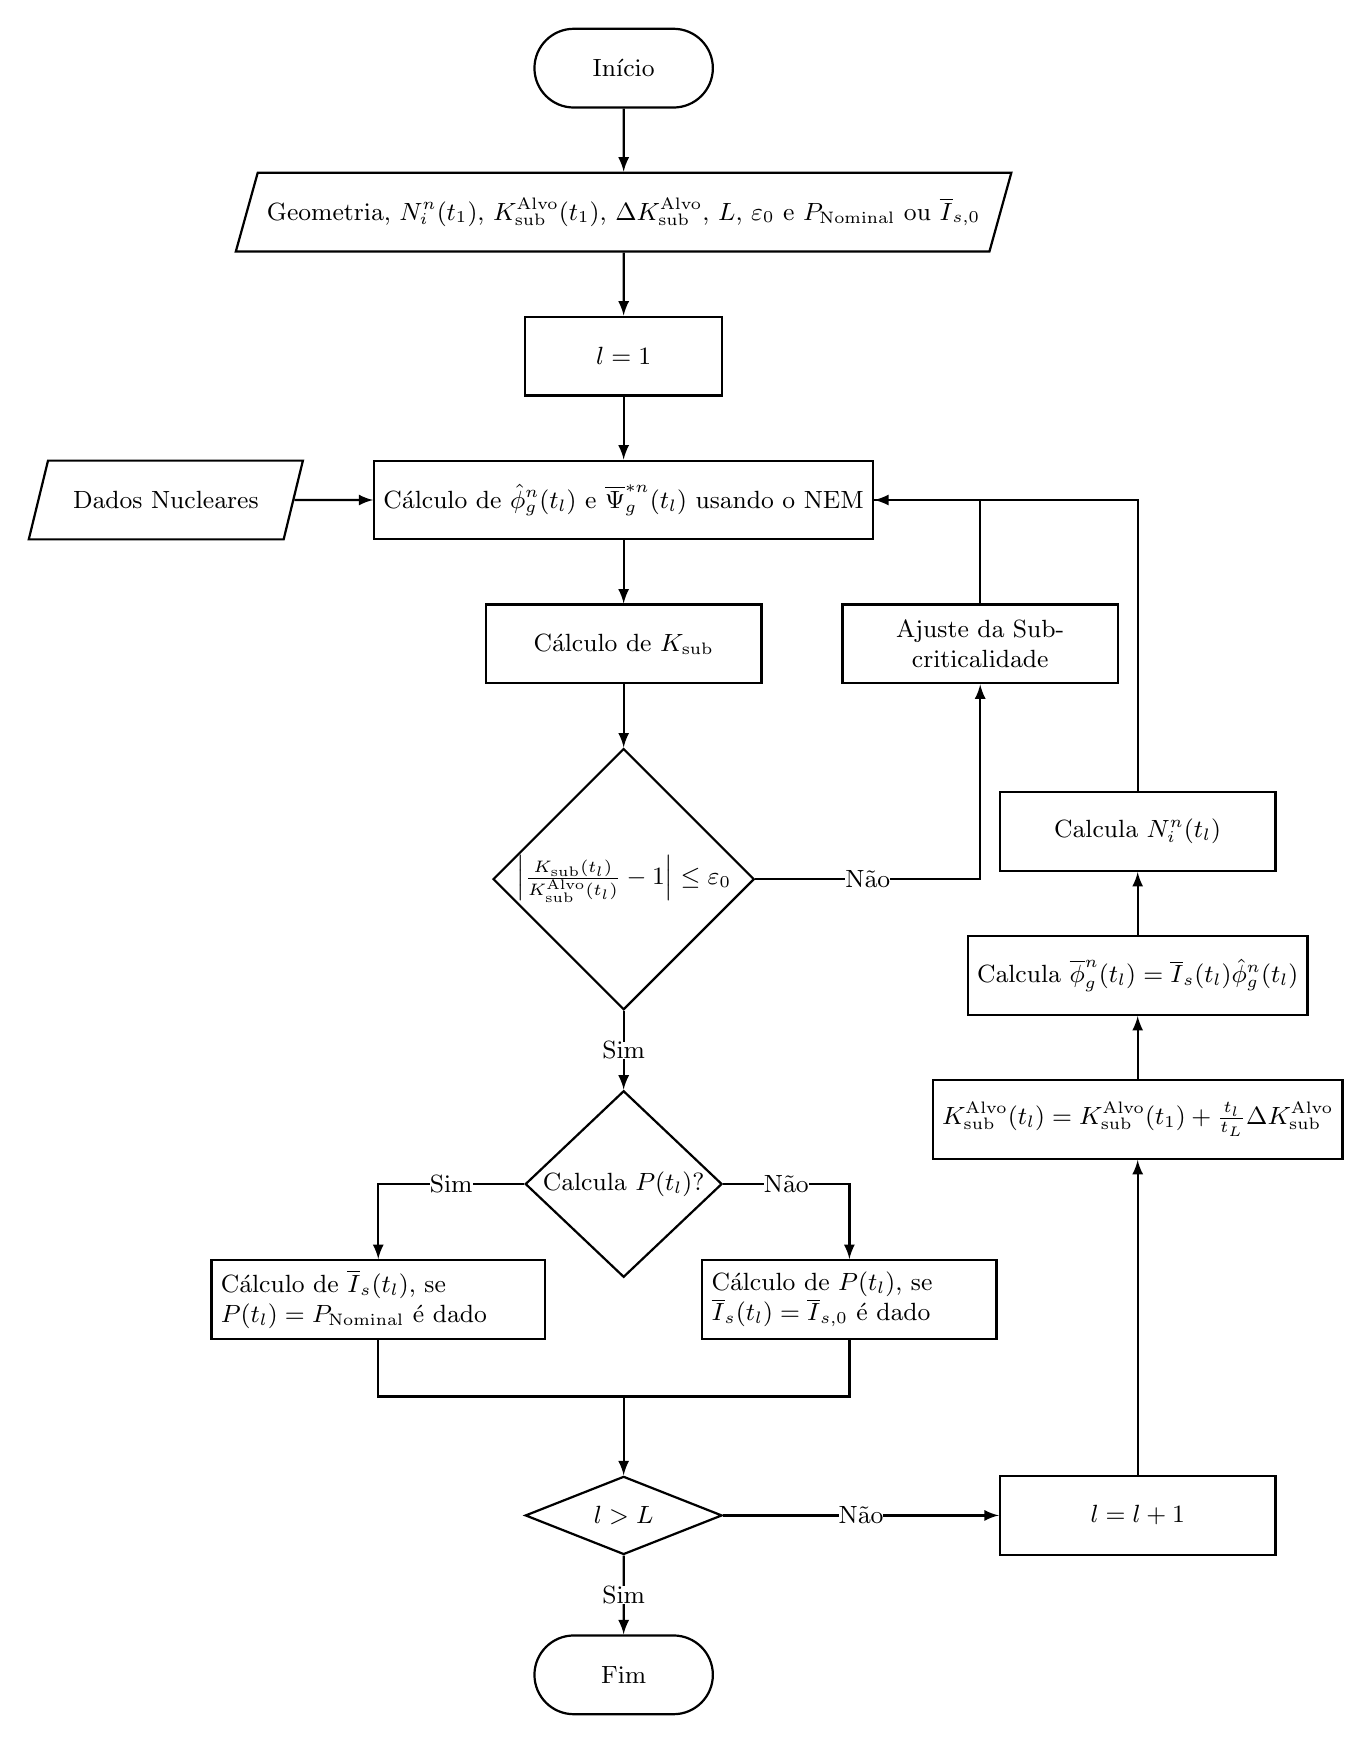
\begin{tikzpicture}[font=\small,thick]
 
% Start block
\node[draw,
    rounded rectangle,
    minimum width=2.5cm,
    minimum height=1cm] (block1) {Início};
 
% Voltage and Current Measurement
\node[draw,
    trapezium, 
    trapezium left angle = 65,
    trapezium right angle = 115,
    trapezium stretches,
    below= 0.8cm of block1,
    minimum width=3.5cm,
    minimum height=1cm
] (block2) { Geometria, $N_i^n{(t_1)}$, $K_{\text{sub}}^\text{Alvo}(t_1)$, $\Delta K_{\text{sub}}^\text{Alvo}$, $L$, $\varepsilon_0$ e $P_\text{Nominal}$ ou $\overline{I}_{s,0}$};
 
% Power and voltage variation
\node[draw,
    below=0.8cm of block2,
    minimum width=2.5cm,
    minimum height=1cm
] (block3) { $l=1$};

% Power and voltage variation
\node[draw,
    below=0.8cm of block3,
    minimum width=3.5cm,
    minimum height=1cm
] (block4) {Cálculo de $\hat{\phi}_g^n(t_l)$ e $\overline{\Psi}_g^{*n}(t_l)$ usando o NEM};

% Voltage and Current Measurement
\node[draw,
    trapezium, 
    trapezium left angle = 65,
    trapezium right angle = 115,
    trapezium stretches,
    left=of block4,
    minimum width=3.5cm,
    minimum height=1cm
] (block21) {Dados Nucleares};

% Power and voltage variation
\node[draw,
    below=0.8cm of block4,
    minimum width=3.5cm,
    minimum height=1cm
] (block5) {Cálculo de $K_{\text{sub}}$};
    
% Conditions test
\node[draw,
    diamond,
    below=0.8cm of block5,
    minimum width=2.5cm,
    inner sep=0] (block6) {$\left|\frac{K_{\text{sub}}(t_l)}{K_{\text{sub}}^\text{Alvo}(t_l)} -1 \right| \le \varepsilon_0$};
    
    
% Conditions test
\node[draw,
    diamond,
    below=of block6,
    minimum width=2.5cm,
    inner sep=0] (block7) {Calcula $P(t_l)$?};   

% Power and voltage variation
\node[draw,
    below left=0.5cm of block7,
    minimum width=3.5cm,
    minimum height=1cm,
    text width=4cm
] (block8) {Cálculo de $\overline{I}_s(t_l)$, se $P(t_l)=P_\text{Nominal}$ é dado};  

% Power and voltage variation
\node[draw,
    below right=0.5cm of block7,
    minimum width=3.5cm,
    minimum height=1cm,
    text width=3.5cm
] (block9) {Cálculo de $P(t_l)$, se $\overline{I}_s(t_l)=\overline{I}_{s,0}$ é dado};  

% Power and voltage variation
\node[draw,
    right= 1cm of block5,
    minimum width=3.5cm,
    minimum height=1cm,
    text width=3cm,
    text centered
] (block17) {Ajuste da Subcriticalidade};  

\node[coordinate,below=1.5cm of block7] (block16) {};

% Conditions test
\node[draw,
    diamond,
    below= of block16,
    minimum width=2.5cm,
    inner sep=0] (block10) {$l>L$};
  

%\node[coordinate,right=0.5cm of block17] (block18) {};
    

% Power and voltage variation
\node[draw,
    right=3.5cm of block10,
    minimum width=3.5cm,
    minimum height=1cm
] (block12) {$l=l+1$};

% Power and voltage variation
\node[draw,
    above=4cm of block12,
    minimum width=3.5cm,
    minimum height=1cm
] (block13) {$K_{\text{sub}}^\text{Alvo}(t_l) = K_{\text{sub}}^\text{Alvo}(t_1) + \frac{t_l}{t_L}\Delta K_\text{sub}^\text{Alvo}$}; 

% Power and voltage variation
\node[draw,
    above=0.8cm of block13,
    minimum width=3.5cm,
    minimum height=1cm
] (block14) {Calcula $\overline{\phi}_g^n(t_l) = \overline{I}_s(t_l)\hat{\phi}_g^n(t_l)$};    


% Power and voltage variation
\node[draw,
    above=0.8cm of block14,
    minimum width=3.5cm,
    minimum height=1cm
] (block18) {Calcula $N_i^n(t_l)$};    
    
% Return block
\node[draw,
    rounded rectangle,
    below=of block10,
    minimum width=2.5cm,
    minimum height=1cm,] (block11) {Fim};
 
% \node[coordinate,below=4.35cm of block4] (block12) {};
 
 
% Arrows
\draw[-latex] (block1) edge (block2)
    (block2) edge (block3)
    (block3) edge (block4)
    (block21) edge (block4)
    (block4) edge (block5)	
    (block5) edge (block6);
 
\draw[-latex] (block6) -- (block7)
    node[pos=0.5,fill=white,inner sep=0]{Sim};
    
\draw[-latex] (block6) -| (block17)
    node[pos=0.25,fill=white,inner sep=0]{Não};    
 
\draw[-latex] (block7) -| (block8)
    node[pos=0.25,fill=white,inner sep=0]{Sim};

\draw[-latex] (block7) -| (block9)
    node[pos=0.25,fill=white,inner sep=0]{Não};

\draw (block8) |- (block16);
 
\draw (block9) |- (block16);

\draw[-latex] (block16) -- (block10);

\draw[-latex] (block10) -- (block11)
    node[pos=0.5,fill=white,inner sep=0]{Sim};

\draw[-latex] (block10) -- (block12)
    node[pos=0.5,fill=white,inner sep=0]{Não};


\draw[-latex] (block12) edge (block13)
              (block13) edge (block14)
              (block18) |- (block4)
              (block17) |- (block4)
              (block14) edge (block18);
%\draw (block17) -- (block18);              
 
\end{tikzpicture}
\vspace{-1cm}
\caption{Fluxograma do algoritmo de solução para determinar o parâmetro $K_{\text{sub}}$.}
\label{chap3:fluxograma}
\end{figure}

    \chapter{Descrição do Sistema ``Admins''}
\label{chap4}

Dado a escolha de um banco de dados em grafo como o Neo4j, o sistema ``Admins'' veio para resolver o problema de ser complicado e pouco seguro gerenciar os dados diretamente através de uma Cypher no banco, sendo facilmente possível realizar consultas muito pesadas, ou que tem consequências difíceis de reverter, de maneira acidental.

Foi então desenvolvido uma interface para usuários interagirem com o banco, podendo criar, editar, conectar e desconectar arbitrariamente nós no banco de dados. Esse sistema foi nomeado de 'admins', graças ao subdomínio utilizado para hospoedá-lo.

\section{Perfis e Listas}

Junto com o time de Design, identificamos uma maneira de entender e visualizar o grafo que está armazenado no banco, dando para cada nó uma página de perfil, que mostra e permite edição de suas propriedades e relações, além de uma página de lista/pesquisa para cada rótulo (relevante) no banco de dados. Endentendo este isomorfismo, conseguimos criar esta interface e permitir os usuários navegarem e editarem o grafo de maneira intuitiva.

\begin{figure}[H]
    \centering
    \includegraphics[width=1.0\linewidth]{Imagens/chap04/perfil-isomorfismo.png}
    \caption{Um \textcolor{green}{\textbf{nó X}} está relacionado à \textcolor{purple}{\textbf{um nó de rótulo Y}}, \textcolor{blue}{\textbf{um de rótulo W}}, e possui relação com \textcolor{orange}{\textbf{três nós de rótulos Z}} no grafo armazenado no banco de dados.}
    \label{fig:isomorphism}
\end{figure}


Temos então as propriedades do nó dono do perfil na parte superior da tela, e diferentes abas (uma para cada tipo de relação que o nó dono possui) na parte inferior, sendo que dentro de cada aba, uma lista de elementos com os nós vizinhos através daquele tipo de relação, com hiperlinks para páginas de perfis de seus vizinhos. Assim conseguimos andar pelo grafo através dos nós e relações, e em cada parada temos ações específicas como edição, criação ou conexão de nós.

Porém para o usuário começar esta navegação, ele precisa primeiro determinar o nó inicial. Essa é a função da chamada página de Lista, que como o nome sugere lista de maneira paginada e com funções de pesquisa os nós de algum rótulo específico, numa lista de elementos similar à uma aba dentro de um perfil. Permitindo agir sobre esses nós, ou entrar na página de perfil de um deles, começando a navegação pelos perfis.

A vantagem dessa modelagem é que conseguimos perceber que toda página de perfil (e de lista) segue a mesma regra, logo o código referente à sua implementação pode ser reutilizado. Ná prática a aplicação consiste em apenas uma página de perfil, e uma página de lista (além da página de login/autenticação), e mapas que definem as especificidades de cada caso, facilitando sua manutenção e minimizando o tamanho do seu código, consequentemente minimizando também bugs em produção.

\section{Arquitetura da Aplicação Cliente}

\subsection{Ações}

\section{Arquitetura do Servidor com endpoint GraphQL}

O frontend, entretando, não se comunica diretamente com o banco de dados, a interface se comunica com uma camada intermediária através de requisições em GraphQL, e esta camada intermediária gera a Cypher resultante, que então é executada no banco de dados. Nesta seção descreveremos como funciona e a arquitetura escolhida para esta camada intermediária, o servidor que disponibiliza a endpoint em Graphql.

 \begin{figure}[H]

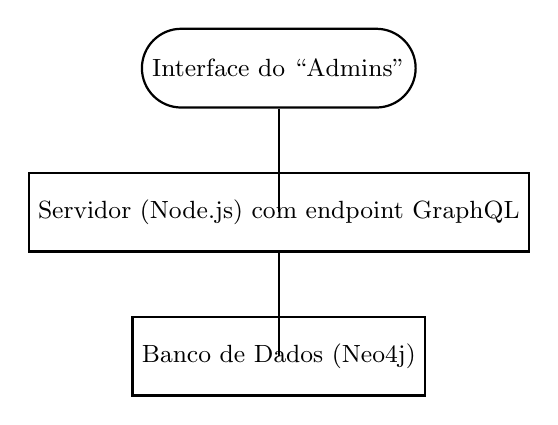
\begin{tikzpicture}[font=\small,thick]
 
% Start block
\node[draw,
    rounded rectangle,
    minimum width=2.5cm,
    minimum height=1cm] (block1) { Interface do ``Admins'' };
 
% Voltage and Current Measurement
\node[draw,
    below=0.8cm of block1,
    minimum width=2.5cm,
    minimum height=1cm
] (block2) { Servidor (Node.js) com endpoint GraphQL };
 
% Power and voltage variation
\node[draw,
    below=0.8cm of block2,
    minimum width=2.5cm,
    minimum height=1cm
] (block3) { Banco de Dados (Neo4j) };

\draw (block1) |- (block2);
\draw (block2) |- (block3);

\end{tikzpicture}
\caption{Fluxograma de comunicação entre partes do sistema }
\label{chap3:fluxograma}
\end{figure}
    \chapter{Sistema em Operação}
\label{chap5}


\section{Jovens Gênios Provedor de Conteúdo LTDA}

A Jovens Gênios surgiu em 2016 com Fernando Costa, aluno da Escola de Química da UFRJ e apaixonado por Educação, procurando soluções de ensino extracurriculares engajantes para seus irmãos mais novos. Seguindo uma lógica "efetual"[1] 
Effectuation: Elements of Entrepreneurial Expertise
, não satisfeito com as soluções existentes,desenvolveu plataformas de apoio ao processo de ensino-aprendizagem embrionárias, tendo os irmãos como primeiros usuários.
Mais tarde, junto com o antigo colega Bernard Caffé, que compartilhava a paixão por educação, tendo experiência como professor e com o estudo de Metodologias Ativas de aprendizado, fundaram a empresa Jovens Gênios, tendo escolas de bairro como seus primeiros clientes.

A experiência foi bem sucedida, sendo hoje, seis anos depois, utilizada por centenas de milhares de usuários/alunos de todo o Brasil, os quais registraram através das plataformas Jovens Gênios centenas de milhões de respostas em questões.

\section{Modelagem do Domínio}

O caso de uso da Jovens Gênios inclui nós das estruturas escolares (Redes de ensino, Escolas, Turmas, Alunos, Professores, Gestores), nós do conteúdo gerado pela empresa (Questões, Resumos, Tópicos, Cursos, Disciplinas), nós das atividades que acontecem nas plataformas (Desafios, Tarefas, Provas Somativas, Provas Diagnósticas, Batalhas, Campeonatos, Aulas Invertidas), e, principalmente, os nós referentes às respostas dos alunos, que conectam o aluno à questão e ao contexto da atividade que levou o aluno àquela questão.

A estrutura em árvore dos tópicos e da estrutura escolar, assim como a facilidade de realizar a manutenção e desenvolver novas funcionalidades utilizando a biblioteca @neo4j/graphql, foram os fatores determinantes para a escolha de um banco em grafo.

\section{Papeis dos Usuários do sistema ``Admins''}

Os seguintes perfis de colaboradores são usuários do sistema ``Admins'' na Jovens Gênios:

\begin{itemize}
    \item Educacional (Responsáveis pelo contato direto com as escolas e definição das turmas)
    \item Suporte (Contato com alunos e professores para esclarecer dúvidas e mapear eventuais problemas)
    \item QA (Controle de qualidade e interface com os desenvolvedores)
    \item Desenvolvedores (Visualizar e realizar eventuais manipulações no banco de dados)
\end{itemize}


    \chapter{Conclusões}
\label{chap6}
 \section{Resultados}
1-2 parag

Com a implentação do sistema admins usuarios interagiram de maneira mais rapida, algun dado, produtividade, retorno pessoal

curto periodo de aprendizado 

\begin{figure}
    \centering
    \includegraphics[width=1\linewidth]{image.png}
    \caption{PLACEHOLDER }
    \label{fig:enter-label}
\end{figure}

são diversas opções de busca gero engessado - devido à natureza do grafo, sempre tem diversas maneiras de alcançar um mesmo objetivo (conectar por um lado ou pelo outro, pesquisar em mais de um lugar, e etc)

 \section{Trabalhos Futuros}

Dentre as possíveis implementações adicionais podemos citar:
\begin{itemize}
    \item Apesar de medidas de segurança para garantir que apenas usuários autorizados  ainda é interessante tornar o sistema mais robusto com medidas adicionais de prevenção de acesso à base de dados por usuários de perfil inadequado
- sistema mais robusto
    \item Gerar automaticamente os arquivos que definem as requisições .gql com as informações retornadas pela InstrospectionQuery. A configuração prévia da estrutura de arquivos pode ser um ponto de dor para o desenvolvimento ~
    \item Desenvolver um sistema de interface 'perfil e listas' de maneira compatível à disponibilizar no Neo4j Developer Graph Apps 
\end{itemize}




  \backmatter
  %\nocite{*}
  \bibliographystyle{coppe-unsrt}
  \bibliography{thesis}
  \appendix
  \chapter{Código Fonte Aberto}
\label{apendice}


\definecolor{lightgray}{rgb}{.9,.9,.9}
\definecolor{darkgray}{rgb}{.4,.4,.4}
\definecolor{purple}{rgb}{0.65, 0.12, 0.82}

\end{document}
